\documentclass[11pt]{article}
\usepackage[utf8]{inputenc}
\usepackage[T1]{fontenc}
\usepackage[margin=1in]{geometry}
\usepackage{amsmath,amssymb,amsthm}
\usepackage{booktabs}
\usepackage{array}
\usepackage{url}
\usepackage{microtype}
\usepackage{graphicx}
\usepackage{caption}
\usepackage{xcolor}
\usepackage{listings}
\usepackage[hidelinks]{hyperref}
\makeatletter\g@addto@macro{\UrlBreaks}{\do\_\do\.\do\/}\makeatother
\emergencystretch=3em
\tolerance=2000
\newcommand{\nRows}{115}
\newcommand{\nAcc}{106}
\newcommand{\nRef}{9}
\newcommand{\maxErr}{3.1e-10}
\newcommand{\maxInterior}{6.3e-10}
\newcommand{\maxDrift}{9.8e-14}
\newcommand{\expmDiff}{1.0e-13}
\newcommand{\minComp}{-4.6e-18}
\newcommand{\nMoranRuns}{78}
\newcommand{\nWFRuns}{28}

\lstset{basicstyle=\ttfamily\scriptsize,columns=fullflexible,keepspaces=true,breaklines=true,
  frame=single,framesep=3pt,xleftmargin=4pt,xrightmargin=4pt,upquote=true,
  keywordstyle=\bfseries,morekeywords={theorem,lemma,def,noncomputable,abbrev,structure,where,fun,Prop,axiom},
  escapeinside={(*@}{@*)}}
\newtheorem{theorem}{Theorem}
\newtheorem{lemma}[theorem]{Lemma}
\theoremstyle{remark}
\newtheorem{remark}[theorem]{Remark}
\newcommand{\R}{\mathbb{R}}
\newcommand{\tier}[1]{\textsf{[#1]}}
\newcommand{\lean}[1]{\texttt{#1}}
\newcommand{\Pn}{P^{n}}
\makeatletter\newcommand{\tabinput}[1]{\@@input #1 }\makeatother

\title{Fixation probabilities as absorption limits of matrix powers, kernel-checked:\\
neutral Wright--Fisher, the Moran model with selection, the Price equation,\\
and a fail-closed CVODE certificate}
\author{Xavier Callens (SocrateAI Lab)\thanks{AI-assistance disclosure: this preprint, its Lean files, its code and
its ledger were produced by AI agents (Claude, Anthropic) under the author's direction. The author is responsible for
the content. No human expert has reviewed it.}}
\date{Preprint v1, 2026-10-25 (revised after an independent AI audit)}
\hypersetup{pdftitle={Fixation probabilities as absorption limits of matrix powers, kernel-checked},
  pdfauthor={Xavier Callens}}

\begin{document}
\maketitle
\begin{center}\small Not peer reviewed. DOI assigned at deposit.\end{center}

\noindent\textbf{AI-assistance disclosure.} This preprint, its Lean code, its Rust and Python code and its claim ledger
were produced by AI agents (Claude, Anthropic) under the author's direction. The author is responsible for the content.
No human has audited the Lean statements for adequacy, and no human referee has checked the hand proofs. The Lean files
were compiled by their producer agents and re-compiled at the paper stage by the same AI pipeline. A separate AI agent
then audited the preprint: it recompiled every Lean module from source in its own build directory (not the producer's
\texttt{.olean} files), ran its own axiom audit and its own planted controls, reproduced the CVODE results byte for byte,
re-derived the numbers, hand proofs and citations, and gave the verdict ACCEPT\_WITH\_CORRECTIONS with no blocking issue
(\texttt{AUDIT.md}; this version applies its corrections, see \texttt{REVISION.md}). That auditor is an AI of the same model
family as the producer, so this is an independent recompile and not a human audit. Three things changed after the audit
and were re-checked only by the revising agent: a doc comment in \lean{FixationDataCert.lean} (recompiled, rc~0, same axiom
lines), the Rust crate (a componentwise non-negativity check, commit \texttt{cda9a90}), and, as a consequence, \texttt{results.jsonl}
(regenerated: one added field and one \texttt{null}; the auditor's byte-for-byte reproduction refers to the earlier file, and every other field is unchanged). Treat every Tier~A statement
below as ``kernel-checked, statement adequacy not audited by a human''.

\begin{abstract}
For a stochastic kernel $P$ on $\{0,\dots,N\}$ with absorbing ends we prove in Lean~4 that the $n$-step probability of
being at $N$ converges to $h(i)$, and that of being at $0$ to $1-h(i)$, whenever $h$ is harmonic at the interior states
with boundary values $0$ and $1$ and the one-step variance of $h$ is positive at every interior state. The proof is a
second-moment argument: the interior mass has bounded partial sums, hence tends to $0$, and a squeeze finishes. One
theorem covers two models. For neutral Wright--Fisher, $\Pn(i,N)\to i/N$ (this closes a gap recorded in an earlier
module, which proved only uniqueness of the harmonic function). For the Moran process with fitness $r>0$,
$\Pn(i,N)\to S_i/S_N$ with $S_n=\sum_{k<n}r^{-k}$, that is $(1-r^{-i})/(1-r^{-N})$ for $r\ne1$ and $i/N$ for $r=1$;
the limit $r\to1$ of the closed form is proved too. We also prove the Price equation for a finite population as an
exact identity over any field, and its haploid corollary $\Delta\bar w=\mathrm{Var}_n(w)/\bar w$ for constant type
fitnesses and no transmission bias.

\textbf{Tier A} (Lean 4.34.1, Mathlib only; axioms within \lean{propext}, \lean{Classical.choice}, \lean{Quot.sound};
planted \lean{sorry} and planted-axiom controls caught; kernel-checked positive and negative controls). \textbf{What is
not proved:} the identification of the matrix power $\Pn(i,N)$ with the probability $\mathbb P_i(T_N\le n)$ of a path
measure is the standard definition of the $n$-step law and is not formalised (Tier~C); and the preregistered
``Fisher's theorem in the partial-change reading'' was \emph{not achieved}: only the haploid constant-fitness special case is
proved. \textbf{Tier X:} a new rusty-SUNDIALS crate, \lean{qf-popgen}, integrates the uniformised Kolmogorov equation with
CVODE (BDF, exact Jacobian) behind a \emph{fail-closed} absorption certificate (kernel validity, mass conservation,
componentwise non-negativity, decay of the interior mass, agreement with the target): \nAcc{} accepted runs agree with the closed
forms to $\le\maxErr$ (and with \texttt{scipy.linalg.expm} to $\le\expmDiff$), and all \nRef{} negative controls are
refused. All results are classical; no novelty is claimed, and nothing here depends on openai/math results.
\end{abstract}

\paragraph{Tiers.} \tier{A}: kernel-checked Lean, axioms within the allowlist, planted controls caught.
\tier{L}: a cited source, quoted in the ledger (prose as extracted, mathematics transcribed linearly, elisions marked),
pinned to a page. \tier{C}: an argument or human proof that is not machine-checked. \tier{X}: floating-point
exploration, which never supports a claim. Identifiers such as \texttt{PG-A-0001} refer to \texttt{ledger/ledger.json}
(Section~\ref{sec:ledger}). A Tier~A tag attaches to the Lean statement, never to its biological gloss. Status words:
every module was compiled by its producer, re-compiled by the same AI pipeline, and then \emph{recompiled from source by a
separate AI auditor} (own build directory, own axiom audit, own planted controls; verdict ACCEPT\_WITH\_CORRECTIONS); the one module
imported from earlier work (\texttt{PopGenWrightFisher.lean}, ``H11'') was likewise recompiled by a separate AI verifier. No module has
had a human audit, and the auditor shares the producer's model family.

\section{Setting}\label{sec:setting}
A population of $N$ individuals contains $i$ mutants. A \emph{kernel} $P$ is an $(N+1)\times(N+1)$ matrix with
non-negative entries and unit row sums; \emph{$0$ and $N$ are absorbing} if rows $0$ and $N$ are the point masses
$\delta_0,\delta_N$. The $n$-step kernel is defined by the Chapman--Kolmogorov recursion
$P^{0}=I$, $P^{n+1}(i,j)=\sum_k P^{n}(i,k)P(k,j)$ (\lean{kPow} in Lean), the interior mass is
$I_n(i)=\sum_{0<k<N}P^{n}(i,k)$, and $h$ is \emph{interior-harmonic} if $\sum_jP(i,j)h(j)=h(i)$ for $0<i<N$.
Listing~\ref{lst:absdefs} gives these definitions verbatim up to glyph rendering (the listings replace a few Unicode symbols by \LaTeX{} glyphs, the symbols for the reals, the neighbourhood filter and negation appear as $\mathbb{R}$, $\mathcal N$, $\neg$; the Lean files in the repository are the reference).

\lstinputlisting[caption={Chains on \lean{Fin (N+1)}: definitions (\texttt{Absorption.lean}, verbatim up to glyph rendering).},label=lst:absdefs]{gen/abs_defs.lst}

The two models are the neutral Wright--Fisher kernel $\mathrm{wfP}_N(i,j)=\binom Nj(i/N)^j(1-i/N)^{N-j}$ (imported unchanged
from the earlier module H11) and the Moran process with fitness $r>0$: with $i$ mutants, one individual is chosen to
reproduce with probability proportional to fitness and one uniformly at random dies, so the mutant count moves up with
probability $p_i$, down with probability $q_i$ and stays otherwise,
\[
p_i=\frac{r i}{r i+N-i}\cdot\frac{N-i}{N},\qquad q_i=\frac{N-i}{r i+N-i}\cdot\frac{i}{N}.
\]
Keller and U\u{g}urlu write the same rates as $p^{+}(j)=\frac{r}{1+(r-1)j/n}\frac jn\frac{n-j}n$ and
$p^{-}(j)=\frac{1}{1+(r-1)j/n}\frac{n-j}n\frac jn$, ``the individual to be replaced [being] chosen uniformly at random''
\tier{L, PG-L-0001}; the equality is a one-line computation, $\frac{r j/n}{1+(r-1)j/n}=\frac{r j}{rj+n-j}$
\tier{C, PG-C-0004}. Their fixation probabilities are $\varrho_i=i/n$ ($r=1$) and
$(1-1/r^{i})/(1-1/r^{n})$ ($r\ne1$), derived by optional stopping on the martingale $r^{-M_k}$ \tier{L, PG-L-0002}.
Our route avoids a path measure and works on matrix powers (Listing~\ref{lst:moran-defs}).

\lstinputlisting[caption={The Moran model and its fixation function (\texttt{MoranModel.lean}, verbatim up to glyph rendering).},label=lst:moran-defs]{gen/moran_defs.lst}

\paragraph{Bridge to probability (Tier C, PG-C-0001).} $\Pn(i,N)$ is by definition the $n$-step transition probability
$\mathbb P_i(X_n=N)$ of the chain with kernel $P$; since $N$ is absorbing, $\{X_n=N\}=\{T_N\le n\}$, so
$\Pn(i,N)=\mathbb P_i(T_N\le n)$, which is consistent with the kernel-checked monotonicity of $\Pn(i,N)$ in $n$. The limit is
therefore the fixation probability $\mathbb P_i(T_N<\infty)$. This identification is standard and is \emph{not} a
Lean statement here: no path space is built. Mathlib has an Ionescu--Tulcea construction, \lean{ProbabilityTheory.Kernel.traj}, which Marion describes as integrated into Mathlib
\tier{L, PG-L-0003}; that it is present in the pinned build is a repository fact (declared in \texttt{Mathlib/Probability/Kernel/IonescuTulcea/Traj.lean}, line~518, found by
grep in the audit), not a citation. It could carry the bridge; we do not use it. Wording used throughout: ``the $n$-step absorption probability
at $N$ converges to\dots; kernel-checked''.

\section{Step-by-step human demonstration}\label{sec:human}
This section is for a strong undergraduate. Each step states a fact, proves it by hand \tier{C, PG-C-0003}, and names
the Lean declaration that checks the matching statement \tier{A}. Let $P$ be a kernel on $\{0,\dots,N\}$, $N>0$, with
$0,N$ absorbing, and let $h$ be interior-harmonic with $h(0)=0$, $h(N)=1$ and
\[
v(k)=\sum_jP(k,j)\bigl(h(j)-h(k)\bigr)^2>0\quad(0<k<N).
\]

\paragraph{Step 1: martingale identity \tier{A, PG-A-0001}.} \emph{Claim:} $P^nh=h$ for all $n$, i.e.
$\sum_jP^n(i,j)h(j)=h(i)$. \emph{Proof.} At an absorbing end the row is a point mass, so $(Ph)(0)=h(0)$ and
$(Ph)(N)=h(N)$; with interior harmonicity, $Ph=h$ everywhere. Then $P^{n+1}h=P^n(Ph)=P^nh$, and induction on $n$.
The same argument with $h\equiv1$ shows that rows of $P^n$ sum to $1$; non-negativity of $P^n$ is induction on the recursion.
Lean: \lean{kPow\_harmonic}, \lean{kPow\_rowSum}, \lean{kPow\_nonneg}.

\paragraph{Step 2: second-moment identity \tier{A, PG-A-0001}.} \emph{Claim:}
$\sum_jP(k,j)h(j)^2=h(k)^2+v(k)$. \emph{Proof.} Expand $(h(j)-h(k))^2=h(j)^2-2h(k)h(j)+h(k)^2$ and use
$\sum_jP(k,j)=1$ and $\sum_jP(k,j)h(j)=h(k)$. Lean: \lean{second\_moment}.

\paragraph{Step 3: the interior mass is summable \tier{A, PG-A-0001}.} \emph{Claim:} $I_n(i)\to0$. \emph{Proof.} Let
$\varepsilon=\min_{0<k<N}v(k)>0$ (a minimum over finitely many positive numbers). By Step~2, pointwise
$P(h^2)\ge h^2+\varepsilon\,\mathbf 1_{\rm int}$: at interior $k$ this is $v(k)\ge\varepsilon$, and at an end state both sides
equal $h(k)^2$. Apply $P^m$, whose entries are $\ge0$: $P^{m+1}(h^2)\ge P^m(h^2)+\varepsilon I_m$. Summing over $m<n$,
\[
\varepsilon\sum_{m<n}I_m(i)\le P^n(h^2)(i)-h(i)^2\le\sum_jh(j)^2=:G,
\]
since the rows of $P^n$ sum to $1$. The partial sums of the non-negative series $\sum_mI_m(i)$ are bounded by $G/\varepsilon$,
so it converges and its terms tend to $0$. Lean: \lean{interiorMass\_tendsto\_zero}.

\paragraph{Step 4: the squeeze \tier{A, PG-A-0001}.} \emph{Claim:} $\Pn(i,N)\to h(i)$ and $\Pn(i,0)\to1-h(i)$.
\emph{Proof.} Put $H=\sum_j|h(j)|$. For every state $j$, $|h(j)-\mathbf 1_{j=N}|\le H\mathbf 1_{\rm int}(j)$: at $0$ and $N$
the left side is $0$; at an interior state it is at most $|h(j)|\le H$. Applying $P^n(i,\cdot)$ (non-negative weights) and
Step~1,
$|h(i)-\Pn(i,N)|\le H\,I_n(i)\to0$. Finally $\Pn(i,0)+\Pn(i,N)+I_n(i)=1$ (Lean: \lean{mass\_split}), so
$\Pn(i,0)=1-\Pn(i,N)-I_n(i)\to1-h(i)$. Lean: \lean{absorption\_tendsto}, \lean{fixation\_limit}.

\paragraph{Step 5: uniqueness, and monotonicity \tier{A, PG-A-0001}.} If $g$ is another interior-harmonic function with
$g(0)=0$, $g(N)=1$, then Steps~1 and~4 apply to $g$ with the \emph{same} $I_n\to0$ (it depends on $h$ only through
$v>0$), so $\Pn(i,N)\to g(i)$ as well; limits are unique, hence $g=h$. This replaces the maximum principle used for
Wright--Fisher in H11. And $P^{n+1}(i,N)=\sum_kP^n(i,k)P(k,N)\ge P^n(i,N)P(N,N)=P^n(i,N)$.
Lean: \lean{harmonic\_unique\_of\_var}, \lean{kPow\_last\_mono}.

\lstinputlisting[caption={The general theorem and its main lemmas (\texttt{Absorption.lean}, statements verbatim up to glyph rendering, proofs elided).},label=lst:absthms]{gen/abs_thms.lst}

\paragraph{Step 6: neutral Wright--Fisher \tier{A, PG-A-0002}.} Take $h(j)=j/N$. It is harmonic because the binomial mean is
$\sum_j\binom Nj x^j(1-x)^{N-j}\,j/N=x$ at $x=k/N$ (H11's \lean{frac\_harmonic}). At interior $k$, the jump to $0$
alone contributes $P(k,0)(k/N)^2=(1-k/N)^N(k/N)^2>0$ to $v(k)$, so $v(k)>0$. Steps~1--5 give $\Pn(i,N)\to i/N$ and
$\Pn(i,0)\to1-i/N$.

\lstinputlisting[caption={Wright--Fisher: variance and the limit (\texttt{WrightFisherFixation.lean}, statements verbatim up to glyph rendering).},label=lst:wf]{gen/wf.lst}

\paragraph{Step 7: the Moran kernel is an absorbing chain \tier{A, PG-A-0003, PG-A-0004}.} The ratio of the rates is
$p_i/q_i=r$ (\lean{moranUp\_eq}). The stay probability is
$1-p_i-q_i=\frac{ri^2+(N-i)^2}{(ri+N-i)N}\ge0$ (\lean{moran\_stay\_nonneg}); so $P$ is stochastic, and $p_0=q_0=p_N=q_N=0$ makes
$0,N$ absorbing.

\paragraph{Step 8: the first-step equation \tier{A, PG-A-0003}.} Let $S_n=\sum_{k<n}r^{-k}$ and $h(i)=S_i/S_N$. Then
$h(i+1)-h(i)=r^{-i}/S_N$. The interior harmonic equation $p_ih(i+1)+q_ih(i-1)+(1-p_i-q_i)h(i)=h(i)$ is equivalent to
$p_i\,(h(i+1)-h(i))=q_i\,(h(i)-h(i-1))$, i.e. $p_i\,r^{-i}=q_i\,r^{-(i-1)}$, which is $p_i=rq_i$. Lean:
\lean{moranFix\_harmonic\_nat}. The one-step variance at interior $i$ is at least $p_i(r^{-i}/S_N)^2>0$ because
$p_i>0$ for $0<i<N$ (\lean{moran\_var\_pos\_nat}). Steps~1--5 give, for every $r>0$ and $0<N$
(\lean{moran\_fixation\_limit}, \lean{moran\_fixation\_unique}),
\[
\Pn(i,N)\longrightarrow\frac{S_i}{S_N},\qquad \Pn(i,0)\longrightarrow1-\frac{S_i}{S_N}.
\]

\paragraph{Step 9: closed forms and the neutral limit \tier{A, PG-A-0003, PG-A-0004}.} For $r\ne1$, with $\rho=1/r\ne1$,
the geometric sum gives $S_n=(1-\rho^n)/(1-\rho)$ and so $S_i/S_N=(1-r^{-i})/(1-r^{-N})$
(\lean{moranFix\_closed}, \lean{moran\_fixation\_limit\_closed}). For $r=1$, $S_n=n$ and the value is $i/N$
(\lean{moranFix\_neutral}, \lean{moran\_fixation\_limit\_neutral}); this also shows that neutral Moran and neutral
Wright--Fisher have the same limit although they are different chains. The closed form is continuous at $r=1$: each
$S_n(r)$ is a finite sum of continuous functions with $S_N(1)=N>0$, so
$(1-r^{-i})/(1-r^{-N})\to i/N$ as $r\to1$, $r\neq1$ (\lean{moran\_closed\_tendsto\_neutral}). That settles the
``neutral limit'' as a proof rather than a spot check.

\lstinputlisting[caption={Moran lemmas (\texttt{MoranModel.lean}, statements verbatim up to glyph rendering).},label=lst:moran-lem]{gen/moran_lemmas.lst}
\lstinputlisting[caption={Moran chain theorems (\texttt{MoranFixation.lean}, statements verbatim up to glyph rendering).},label=lst:moran-thm]{gen/moran_thms.lst}

\paragraph{Step 10: the Price equation \tier{A, PG-A-0005}.} A finite population has types $i\in s$ with abundance
$n_i$, fitness $w_i$ (offspring per individual), parental trait $z_i$ and mean offspring trait $z'_i$. Write
$M=\sum n_i$, $A=\sum n_iw_i$, $B=\sum n_iz_i$, $C=\sum n_iw_iz_i$, $D=\sum n_iw_iz'_i$. Then
$\bar w=A/M$, $\bar z=B/M$ and the offspring-generation mean is $\bar z'=D/A$; this definition is the modelling
assumption. Moreover $\mathrm{Cov}_n(w,z)=\frac1M\sum n_i(w_i-\bar w)(z_i-\bar z)=(C-AB/M)/M$ and
$\mathbb E_n[w\,\Delta z]=(D-C)/M$. Hence, if $M\ne0$ and $A\ne0$,
\[
\bar w\,(\bar z'-\bar z)=\frac AM\Bigl(\frac DA-\frac BM\Bigr)=\frac DM-\frac{AB}{M^2}
=\mathrm{Cov}_n(w,z)+\mathbb E_n[w\,\Delta z].
\]
Lean: \lean{price\_equation} (any field, any \lean{Finset} of types; proof: expand the two numerators into the five raw
sums, then \lean{field\_simp; ring}), \lean{wcov\_eq\_moment}, and \lean{price\_equation\_pos} over $\R$ under
$s\ne\emptyset$, $n_i>0$, $w_i>0$.

\paragraph{Step 11: the haploid selection increment \tier{A, PG-A-0006}.} Set the trait equal to fitness, $z=w$, and assume
no transmission bias, $z'=w$ (clonal types, constant fitnesses, no mutation). The transmission term
$\mathbb E_n[w(w-w)]$ is identically $0$, so $\bar w(\bar w'-\bar w)=\mathrm{Var}_n(w)$, i.e.
$\Delta\bar w=\mathrm{Var}_n(w)/\bar w\ge0$ (\lean{fisher\_haploid}, \lean{fisher\_haploid\_div},
\lean{fisher\_haploid\_nondecreasing}, \lean{fisher\_haploid\_pos}). This is LaGatta's eq.~(2.27)
with its environmental term set to zero \tier{L, PG-L-0004}, and the discrete analogue of Baez's remark that
$d\bar f/dt=\mathrm{Var}(f)$ when the fitness functions are constant \tier{L, PG-L-0005}.

\begin{remark}[Scope of Step 11, Tier C, PG-C-0005]
This is \emph{not} Fisher's fundamental theorem in the Price~(1972)/Ewens/Edwards partial-change reading, which concerns
the change ``due to natural selection'' with additive genetic variance, and it is not the diploid multi-allele case. Price's
statement that the theorem is about the fraction of the change due to selection is quoted by LaGatta (p.~4); Baez records that the naive
reading holds only under very restrictive conditions. The preregistered item \texttt{fisher\_general} (prior $0.35$) was
\textbf{not achieved}; negative results are reported.
\end{remark}

\lstinputlisting[caption={Price: definitions (\texttt{Price.lean}, verbatim up to glyph rendering).},label=lst:pricedefs]{gen/price_defs.lst}
\lstinputlisting[caption={Price equation and the haploid increment (statements verbatim up to glyph rendering, proofs elided).},label=lst:pricethms]{gen/price_thms.lst}

\paragraph{Crosswalk to the Genetic repository \tier{A, PG-A-0007; C, PG-C-0007}.} The module
\lean{ProgPopGen.Price.Alix} copies \lean{meanFit} and \lean{selectP} verbatim from
\texttt{SocrateAI-Scientific-Genetic/formal/ANSE/AlixPopulationGenetics.lean} and restates two of its three H12 theorems with
identical statement text (Listing~\ref{lst:alix}): the first is \emph{derived from the multi-type} \lean{fisher\_haploid\_div}
at \lean{Fin 2}, the second is the \lean{wvar} definition at \lean{Fin 2}. The match is textual only: no Lean term links the two namespaces, and the
module was compiled only under the AutoevolveAI pin, not inside the Genetic repository's own build. That repository contains no
Price-equation result (whole-repository search; absence by search).

\lstinputlisting[caption={Crosswalk statements (\texttt{Price.lean}, namespace \lean{ProgPopGen.Price.Alix}, verbatim up to glyph rendering).},label=lst:alix]{gen/alix.lst}

\section{The Lean formalization}\label{sec:lean}
\paragraph{Files and compile records.} Everything is compiled with the pinned toolchain (Lean 4.34.1, Mathlib
\texttt{d13f23b7}), through \texttt{scripts/certified\_numerics/lean\_pinned.py}, with \lean{\#print axioms} for every claimed
declaration. Table~\ref{tab:src} lists the files, their sha256 prefixes (full hashes in the ledger evidence), the exit code of
the latest recompile and the number of \lean{\#print axioms} lines; each of the 11 compiles returned rc~0 with no errors (the \lean{FixationDataCert.lean} row is the recompile after the doc-comment fix of this revision; the independent auditor recompiled the earlier text with the same axiom lines) (the producer transcripts of \texttt{Absorption} and \texttt{MoranModel} show
deprecation warnings for \lean{if\_pos}/\lean{if\_neg}-style lemma names; the controls files show the expected \lean{sorry} warning), and the
axiom lines are identical to the producer transcripts. The claimed files contain no \lean{sorry}, \lean{admit}, \lean{native\_decide} or \lean{axiom}
token (whole-word grep over the claimed and check-only files; the planted controls are in separate files, and two doc-comment lines mention the words, \texttt{FixationDataCert.lean} line~15 and \texttt{MoranModel.lean} line~237).

\begin{table}[ht]\centering\small
\tabinput{gen/table_sources.tex}
\caption{Lean sources (\texttt{formal\_cert/Programmes/PopGen/}; module names are \texttt{Programmes.PopGen.}$\langle$role$\rangle$). All compiles rc~0; the ``axiom lines'' are
\lean{\#print axioms} outputs, each exactly \lean{[propext, Classical.choice, Quot.sound]} for a claimed declaration; the two lines of each
planted-controls file are the planted \lean{sorry} and planted axiom, deliberately outside the allowlist.}\label{tab:src}
\end{table}

\paragraph{Axiom footprint.} Every claimed theorem prints \lean{[propext, Classical.choice, Quot.sound]}. Example, verbatim from the
\texttt{MoranFixation.lean} transcript:

\begin{lstlisting}[basicstyle=\ttfamily\scriptsize]
'ProgPopGen.moran_fixation_limit' depends on axioms: [propext, Classical.choice, Quot.sound]
'ProgPopGen.moran_fixation_unique' depends on axioms: [propext, Classical.choice, Quot.sound]
'ProgPopGen.ctl_neg_wrong_limits' depends on axioms: [propext, Classical.choice, Quot.sound]
\end{lstlisting}

\paragraph{Planted controls (caught).} In a separate file that no claimed module imports, \lean{ctl\_sorry} is ``proved'' by
\lean{sorry} and \lean{ctl\_axiom} from a planted axiom; both claim the \emph{wrong} limits $1/7$ and $1/3$ for the Moran chain at
$N=3$, $r=2$, $i=1$ (the kernel-checked limit is $4/7$). The file compiles with rc~0 and exit status is therefore not the gate; the
axiom audit is \tier{A, PG-A-0012}:

\lstinputlisting[caption={Planted controls (\texttt{PopGenProgControls.lean}, verbatim up to glyph rendering).},label=lst:ctl]{gen/controls.lst}
\begin{lstlisting}[basicstyle=\ttfamily\scriptsize]
'ProgPopGenControls.ctl_sorry' depends on axioms: [propext, sorryAx, Classical.choice, Quot.sound]
'ProgPopGenControls.ctl_axiom' depends on axioms: [propext, Classical.choice, ProgPopGenControls.ctl_cheat, Quot.sound]
\end{lstlisting}
Analogous planted pairs for the Price module and for the data-certificate module are in \texttt{PriceControls.lean} and
\texttt{FixationDataCertControls.lean} (the independent auditor also planted a \lean{sorry}, an axiom and a \lean{sorry} hidden in a lemma of its own, all caught by \lean{\#print axioms}, and showed that changing the positive control $4/7$ to $1/3$ is rejected by the kernel) \tier{A, PG-A-0012, PG-A-0014}; their transcripts show \lean{sorryAx} and the planted
\lean{ctl\_cheat} in the same way (Appendix transcripts \texttt{gen/axioms\_controls\_*.txt}).

\paragraph{Negative controls (kernel-checked, Tier A, PG-A-0008).}
\begin{itemize}\setlength\itemsep{0pt}
\item \lean{ctl\_neg\_identity\_no\_absorption}: the identity kernel on $\{0,1,2\}$ is stochastic and absorbing and $j/2$ is harmonic for
 it, yet $P^n(1,2)=0$ for every $n$, so it does not tend to $1/2$. The variance hypothesis of the main theorem cannot be dropped.
\item \lean{ctl\_neg\_flipped\_value}, \lean{ctl\_neg\_flipped\_not\_harmonic}: the exponent-flipped formula
 $(1-r^i)/(1-r^N)$ gives $1/7\ne4/7$ at $N=3,r=2,i=1$ and violates the first-step equation.
\item \lean{ctl\_neg\_neutral\_not\_harmonic}: under selection, $i/N$ violates the first-step equation.
\item \lean{ctl\_neg\_wrong\_limits}: at chain level, $P^n(1,3)$ for $N=3$, $r=2$ tends neither to $1/3$ nor to $1/7$ (it tends to $4/7$).
\item Price: \lean{ctl\_neg\_transmission\_bias} ($\Delta\bar w=-1/2$ but $\mathrm{Var}/\bar w=1/6$, while Price still holds,
 $-3/4=-3/4$) and \lean{ctl\_neg\_missing\_wbar} ($\Delta\bar w=1/6$ but $\mathrm{Var}=1/4$) \tier{A, PG-A-0010}.
\end{itemize}

\lstinputlisting[caption={Negative controls (statements verbatim up to glyph rendering).},label=lst:neg]{gen/neg_ctl.lst}

\paragraph{Positive controls and non-vacuity (Tier A, PG-A-0009, PG-A-0010, PG-A-0011).} Evaluated directly, not through the limit theorems:
Wright--Fisher $N=2$: $P^2(1,2)=3/8$ (not yet the limit $1/2$); Moran $N=2$, $r=2$: $p_1=1/3$, $q_1=1/6$ and $h(1)=2/3$;
$N=3$, $r=2$: $h=(0,4/7,6/7,1)$ with the first-step equation holding; Price with three types: both sides equal $-13/36$.
The hypotheses are satisfiable: \lean{AbsorbingChain (moranP 3 2)} and \lean{AbsorbingChain (wfP 3)} hold, and the earlier
modules H11 and H12 import together with all P7 modules without name clashes.

\section{Numerics and the rusty-SUNDIALS improvement (Tier X)}\label{sec:numerics}
\paragraph{Method.} The \emph{uniformised} continuous-time chain has law $\pi(t)=\pi(0)\exp(t(P-I))$, the linear ODE
$\dot\pi=\pi(P-I)$ with exact Jacobian $J_{jk}=P_{kj}-\delta_{jk}$. Since $\exp(t(P-I))=\sum_n\mathrm{Poisson}(t;n)P^n$,
the absorption mass $\pi_N(t)$ is a Poisson mixture of the $n$-step probabilities $P^n(i,N)$ and converges to the same limit
\tier{C, PG-C-0002}; this link is not formalised, so the numerics test the same closed forms but not the Lean matrix powers.
The new crate \lean{qf-popgen} of rusty-SUNDIALS (branch \texttt{physics/p7-fixation-2026-10-25}, commit
\texttt{cda9a9057ec16820f2e16b560cc0e63cf7eb05b9}, whose parent \texttt{2b716c58fc7175798ad54dd9363938a3df37d9b0} is the commit the audit examined;
base \texttt{7630f7e} = \texttt{origin/main}; not pushed) integrates this with
CVODE (BDF, rtol $10^{-11}$, atol $10^{-15}$, analytic Jacobian), at output times $t=1,2,4,\dots$ until the interior mass is
$\le10^{-9}$.

\paragraph{The improvement: a fail-closed certificate.} \lean{certify\_absorption} returns a value only if \emph{all} of the following hold, and
otherwise an error (\lean{InvalidKernel}, \lean{Solver}, \lean{NonFinite}, \lean{MassDrift}, \lean{NegativeMass}, \lean{NotAbsorbed}, \lean{ValueMismatch}), never a silent pass:
the kernel is non-negative with unit row sums ($10^{-12}$) and absorbing ends; the state stays finite; $|\sum\pi-1|\le10^{-9}$ at every output;
\emph{every component satisfies $\pi_k(t)\ge-10^{-12}$ at every output};
the interior mass has fallen below $10^{-9}$ by $t_{\max}$; and $|\pi_N-\text{target}|\le10^{-8}$.
The componentwise check is the improvement made in this revision: the audit observed that the total-mass and interior-mass tests are signed sums, so a state such as
$(0.5,-0.25,0.25,0.5)$ (total mass $1$, interior mass $0$) would have passed them. It is now refused by \lean{check\_nonnegative} (unit test, Tier~X);
no reported run was affected, and the smallest component seen at any output of any accepted run is $\minComp$. The binary \lean{fixation\_ode} exits
with status 1 if any run is refused or any negative control is accepted. No change was made to LeanFlow in this lane, and no CVODE core code
was altered; the contribution is a new workspace crate.

\paragraph{Runs.} $\nMoranRuns$ Moran runs (the pairs $(N,r)$: $(2,2)$ and $(3,2)$, which reproduce the Lean positive controls; $(10,1.5)$, $(10,0.8)$, $(10,1)$,
$(20,1.2)$, $(30,2)$) and $\nWFRuns$ Wright--Fisher runs ($N=10,20$), each over every interior start $i=1,\dots,N-1$:
\nAcc{} accepted runs in all, targets $S_i/S_N$ or $i/N$. Table~\ref{tab:cvode} summarises them (the row \texttt{wf\_neutral} pools $N=10$ and $N=20$); Figures~\ref{fig:fix}--\ref{fig:res} show the data.

\begin{table}[ht]\centering\scriptsize
\tabinput{gen/table_cvode.tex}
\caption{CVODE absorption runs by case: the largest deviation from the closed form, the largest interior mass at the stopping time, and the longest stopping time.
All are accepted by the certificate (tolerance $10^{-8}$ on the value, $10^{-9}$ on the interior mass).}\label{tab:cvode}
\end{table}

\begin{figure}[ht]\centering
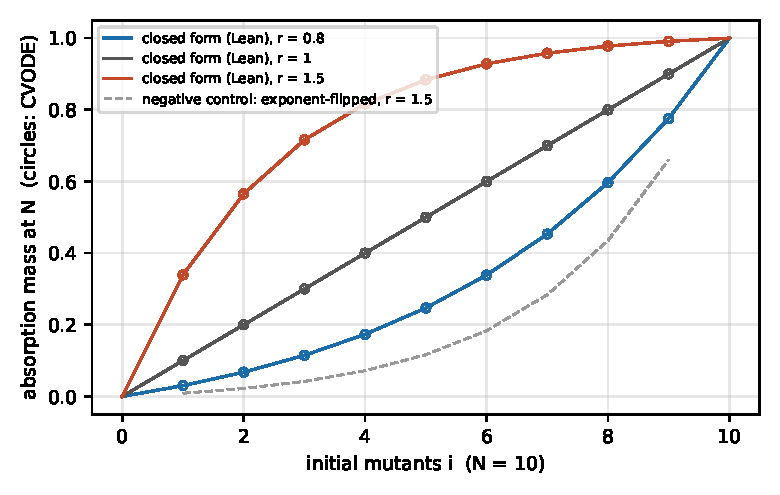
\includegraphics[width=0.62\linewidth]{gen/fig_fixation_vs_i.pdf}
\caption{Moran, $N=10$. Curves: $S_i/S_N$ (the statement kernel-checked in Lean; evaluated here in floating point, Tier~X). Circles: CVODE absorption mass.
Dashed: the exponent-flipped negative control.}\label{fig:fix}
\end{figure}
\begin{figure}[ht]\centering
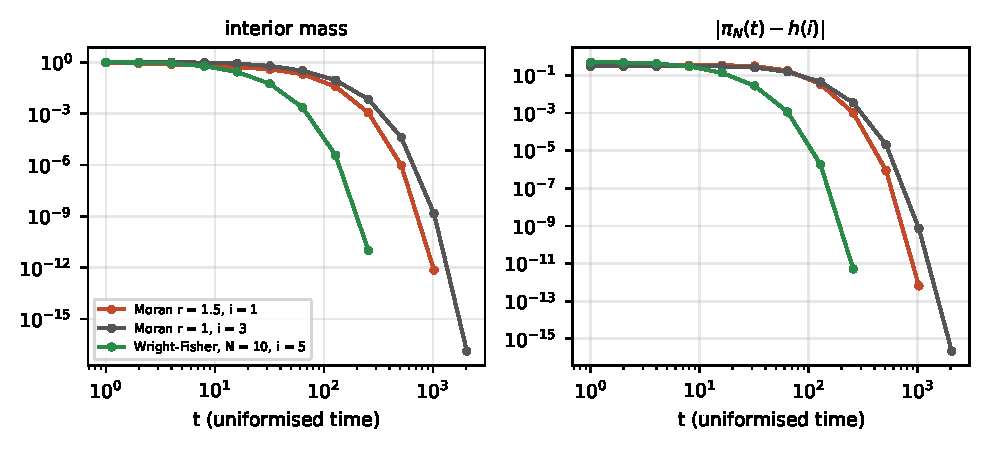
\includegraphics[width=0.85\linewidth]{gen/fig_convergence.pdf}
\caption{Interior mass and absorption error against time for three starts (CVODE, Tier X). The doubling output grid makes the geometric decay look like a
log--log curve.}\label{fig:conv}
\end{figure}
\begin{figure}[ht]\centering
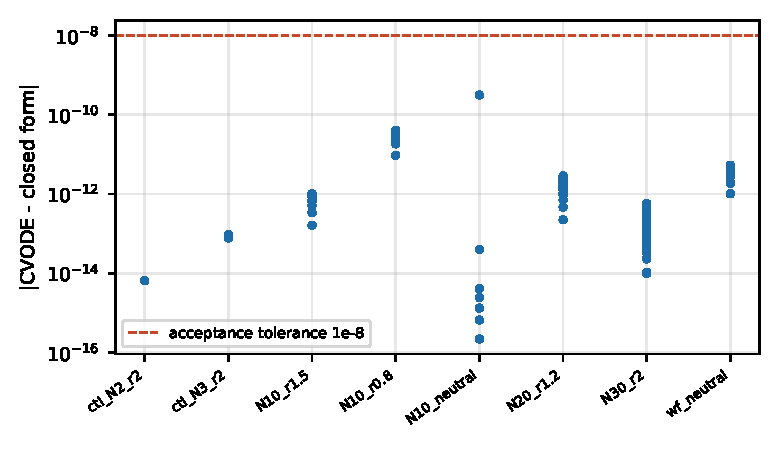
\includegraphics[width=0.55\linewidth]{gen/fig_residuals.pdf}
\caption{Deviation of the CVODE absorption mass from the closed form, all accepted runs, by case (Tier X).}\label{fig:res}
\end{figure}

\paragraph{Controls.} \emph{Positive:} the Lean positive controls $(N,r,i)=(2,2,1)\mapsto2/3$ and $(3,2,\cdot)\mapsto(4/7,6/7)$ are reproduced to $\le10^{-13}$;
the neutral cases give $i/N$. \emph{Negative} (all refused for the stated reason, none accepted; Table~\ref{tab:neg}): the flipped exponent formula and the
neutral $i/N$ at $N=10$, $r=1.5$, $i=1,3,7$ (\lean{ValueMismatch}, the CVODE value being $0.339$, $0.716$, $0.958$ against $0.0088$, $0.042$, $0.284$ and $0.1$, $0.3$, $0.7$); the identity
kernel, a valid absorbing kernel with no absorption flow (\lean{NotAbsorbed}; it mirrors the Lean negative control; it is not a Moran chain, so its fitness field in \texttt{results.jsonl} is \texttt{null}, where the first version of the file carried a meaningless $r=1.5$); a horizon $t\le4$ (\lean{NotAbsorbed}); a corrupted row sum
(\lean{InvalidKernel}); in addition a unit-level control for the new componentwise check (above). \emph{Independent integrator:} the kernels rebuilt separately in \texttt{numpy} and $\exp(t_{\rm stop}(P-I))$ from \texttt{scipy.linalg.expm}
differ from the CVODE absorption mass by at most $\expmDiff$ over all runs \tier{X, PG-X-0003}. The WORK1 cross-check with exact rationals and 60-digit matrix powers
$P^{4096}$ at $N=10$ (errors $\le2\times10^{-61}$ for Wright--Fisher and $\le3.7\times10^{-50}$ for Moran $r=3/2$; $6.6062\times10^{-37}$ at most for $r=1$ on the sampled starts) is recorded as \tier{X, PG-X-0005}.

\begin{table}[ht]\centering\small
\tabinput{gen/table_negative.tex}
\caption{Negative controls of the certificate: 9 of 9 refused.}\label{tab:neg}
\end{table}

\paragraph{Results.} All \nAcc{} runs are accepted: largest deviation $\maxErr$, largest interior mass $\maxInterior$, largest mass drift $\maxDrift$, smallest component $\minComp$ \tier{X, PG-X-0001};
all \nRef{} negative controls are refused \tier{X, PG-X-0002}. These numbers do not support any claim in this paper; they check that an independent integrator and the
Lean closed forms agree.

\paragraph{Data certificates: Lean checks the arithmetic of the decimal literals (Tier A + X).} \lean{FixationDataCert.lean} contains six theorems
$|L-\texttt{moranFix}\ N\ r\ i|<10^{-11}$ whose decimal literals $L$ are the shortest round-trip decimal forms of the \texttt{p\_fix} doubles written by \lean{fixation\_ode} (the JSONL file stores 18 significant digits, for example \texttt{6.66666666666660079e-1}, which round-trips to the literal \texttt{0.6666666666666601}), plus the negative control
that the neutral literal $0.1$ is \emph{not} within $10^{-3}$ of $\texttt{moranFix}\ 10\ (3/2)\ 1$ (Listing~\ref{lst:cert}; \tier{A, PG-A-0013}; provenance of the literals \tier{X, PG-X-0004}).
For the five Moran certificates the decimal literals differ from the exact value by $6.57\times10^{-15}$, $9.55\times10^{-14}$, $7.79\times10^{-14}$, $6.49\times10^{-13}$ and $8.46\times10^{-13}$ (exact rational arithmetic), and in the neutral case the literal \texttt{0.29999999999999977} differs from $3/10$ by $2.30\times10^{-16}$; the float64 difference between \texttt{p\_fix} and the double nearest $3/10$, which is what the file's \texttt{abs\_err} records, is $2.22\times10^{-16}$. All are far inside the proved bounds. The kernel certifies an inequality between a decimal literal and an exact rational, nothing more: it does not certify CVODE, and the literal is not a theorem about a
Markov chain. A planted \lean{sorry}/axiom pair for this module is caught \tier{A, PG-A-0014}.

\lstinputlisting[caption={Data certificates (\texttt{FixationDataCert.lean}, three of the seven statements, verbatim up to glyph rendering; the two certificates and the negative control).},label=lst:cert]{gen/datacert.lst}

\paragraph{Build hygiene.} \texttt{cargo test --release -p qf-popgen -- --test-threads=2} (commit \texttt{cda9a90}): 8 passed, 0 failed (positive: Moran $N=3$, $r=2$, neutral Wright--Fisher, a round-off-level state accepted by the componentwise check; negative: flipped and
neutral targets, identity kernel, corrupted kernel, short horizon, cancelling-entries state refused by the componentwise check; plus a regression check that an accepted run records its minimum component, true by construction). The audit had run the earlier 6 tests at \texttt{2b716c5} (6 passed). \texttt{cargo clippy --workspace --features experimental -- -D warnings}: finished with no warnings;
\texttt{cargo fmt --all --check}: rc~0 \tier{X, PG-X-0007}. The re-run of \lean{fixation\_ode} at \texttt{cda9a90} gives 115 rows, 106 accepted, 9 refused, with every earlier field identical to the first version of the file; the only differences are the added \texttt{min\_component} field and the \texttt{null} fitness of the identity-kernel control.
\section{Limitations}\label{sec:limits}
\begin{itemize}\setlength\itemsep{1pt}
\item \textbf{No path measure.} The Tier~A statements are limits of the matrix powers \lean{kPow}. The identification with $\mathbb P_i(T_N\le n)$ is Tier~C
 (PG-C-0001). The next step is to prove $\texttt{kPow}\,P\,n\,i\,j=(\texttt{Kernel.traj}\ \kappa\ 0\ \delta_i)\{x\mid x_n=j\}$ with the Mathlib construction.
\item \textbf{Moran variant.} The model is the one in which the individual that dies is drawn uniformly from all $N$; other variants (death-birth, graph structure) have different
 rates. The hypotheses are $0<N$ and $0<r$.
\item \textbf{Not formalised:} times to absorption, the diffusion limit (Kimura), mutation, diploid selection, frequency-dependent fitness (here $w$ is fixed within a generation), and
 Fisher's theorem in the partial-change reading (\texttt{fisher\_general}, not achieved).
\item \textbf{Uniqueness route.} For Moran, uniqueness is obtained from uniqueness of limits (Step~5), not from a maximum principle.
\item \textbf{Independent AI recompile, but no human audit.} A separate AI auditor recompiled the modules from source and checked definition fidelity of
 \lean{moranUp}/\lean{moranDown}/\lean{bdP} symbolically against the Keller--U\u{g}urlu rates (PG-C-0004) and the \lean{Fin} indexing of \lean{bdP}; this is an AI judgement from the producer's model family. No human audit exists:
 the ledger gate still flags every Tier~A row for this reason, and the \texttt{audit} fields of the ledger stay null (Section~\ref{sec:ledger}). The auditor did not see the post-audit changes
 (the doc comment and the componentwise check).
\item \textbf{Sources.} Moran (1958), Price (1970) and Price (1972) were \emph{not} read; they appear only as listed in \cite{KU} (p.~18) and \cite{LaG} (p.~69). The novelty
 search was a few \texttt{alphaXiv} queries; absence by search is not proof, and no priority claim is made.
\item \textbf{Genetic crosswalk} is textual (PG-C-0007) and the Price module has not been built inside that repository.
\item \textbf{Numerics} are Tier~X, test the uniformised ODE rather than the Lean matrix powers, and used $N\le30$.
\end{itemize}

\section{Reproducibility}\label{sec:repro}
\begin{itemize}\setlength\itemsep{1pt}
\item \textbf{Lean.} Files under \texttt{formal\_cert/Programmes/PopGen/} of the AutoevolveAI worktree \texttt{openai-math-discovery} (uncommitted at the time of writing; base commit
 \texttt{9d24574}). Full sha256 values are in \texttt{ledger/evidence/}. The independent audit is \texttt{AUDIT.md} and the list of changes made in answer to it is \texttt{REVISION.md}, both in the paper directory. Compile: from the repository root,
 \texttt{taskset -c 4-7 python3 scripts/certified\_numerics/lean\_pinned.py compile FILE --json-out OUT} (pinned Lean 4.34.1 and Mathlib; order: Absorption, WrightFisherFixation,
 MoranModel, MoranFixation, Price, then the import-all and controls files; Absorption, MoranModel, MoranFixation and WrightFisherFixation were also built as importable \texttt{.olean} modules).
\item \textbf{Rust.} \texttt{CARGO\_TARGET\_DIR=\dots{} cargo build --release -j 2 --offline -p qf-popgen}, then \texttt{fixation\_ode OUT\_DIR} writes \texttt{results.jsonl}
 and \texttt{summary.json} (copied to \texttt{data/}). Branch \texttt{physics/p7-fixation-2026-10-25}, commit \texttt{cda9a9057ec16820f2e16b560cc0e63cf7eb05b9} (parent \texttt{2b716c58\dots}, audited); not pushed.
\item \textbf{Figures and tables.} \texttt{gen/gen\_all.py} (figures, run table, independent \texttt{expm} check), \texttt{gen/gen\_listings.py} (verbatim Lean excerpts and axiom
 transcripts from the hashed sources). Run with the repository \texttt{.venv}.
\item \textbf{Earlier work.} Same tier discipline and ledger gate as the companion preprints (DOIs 10.5281/zenodo.23646103, 23646105, 23646107, 23646111, 23646117, which were only reserved when this version was written and resolve once those deposits are published) and the universal-optimality
 textbook (doi:10.5281/zenodo.23295142); the P7 results do not use their theorems.
\end{itemize}

\section{Ledger and gate}\label{sec:ledger}
The ledger has 36 rows: 14 Tier~A, 5 Tier~L, 8 Tier~C, 9 Tier~X; every row has a content-addressed evidence blob. Tier~A rows depend only on Tier~A rows; Tier~C and X rows are never cited as Tier~A support.
The Elenchus gate (\texttt{tools/ledger.py ledger.json --evidence-dir evidence}) reports \textbf{0 blocking findings and 14 flags, exit code 1}: each flag is
\texttt{LEDGER\_UNAUDITED\_TIER\_A}, one per Tier~A row whose statement adequacy no person has audited (verbatim output in \texttt{ledger/gate\_output.txt}). Exit code 1 is the expected outcome while the audit field is null; it is not hidden. The independent AI recompile is recorded as the Tier~X row PG-X-0009 and does not fill any \texttt{audit} field, since it is not a human statement audit.

\begin{table}[ht]\centering\scriptsize
\begin{tabular}{lp{0.78\linewidth}}
\toprule
rows & content\\
\midrule
PG-A-0001..0004 & absorption limit and uniqueness (general); Wright--Fisher; Moran lemmas; Moran chain theorems\\
PG-A-0005..0007 & Price equation; haploid increment; Genetic-repo crosswalk (textual)\\
PG-A-0008..0011 & negative controls; positive controls; Price controls; non-vacuity and import-together\\
PG-A-0012..0014 & planted controls caught (fixation, Price); data-certificate arithmetic; its planted controls\\
PG-L-0001..0005 & Keller--U\u{g}urlu rates and fixation formulas; Marion (\texttt{Kernel.traj}); LaGatta Price/Fisher; Price (1972) via LaGatta and Baez\\
PG-C-0001..0008 & bridge to probability; Poisson link; human proofs; Moran definition fidelity; Price scope (\texttt{fisher\_general} not achieved); no novelty; Genetic note; no openai/math dependence\\
PG-X-0001..0009 & CVODE runs; refused controls; \texttt{expm} check; literal provenance; exact/mpmath; Price numerics; build hygiene; paper-stage recompile (same pipeline); independent AI recompile and audit\\
\bottomrule
\end{tabular}
\caption{Ledger rows.}\label{tab:ledger}
\end{table}

\begin{thebibliography}{99}\small
\bibitem{KU} P.~Keller and M.~U\u{g}urlu, \emph{Fixation probability in Moran-like Processes on graphs}, arXiv:2403.12598v2 [math.PR], 11~Sep.\ 2024 (eqs.\ (3), (4), pp.\ 2--4;
 source typos on pp.\ 2, 3 and 7 not copied; [Mor58] on p.~18).
\bibitem{Mar} E.~Marion, \emph{A Formalization of the Ionescu-Tulcea Theorem in Mathlib}, arXiv:2506.18616v5 [math.PR], 17~Mar.\ 2026 (pp.\ 5, 9, 12).
\bibitem{LaG} T.~LaGatta, \emph{The Mathematics of Evolution: The Price Equation, Natural Selection, and Environmental Change}, arXiv:2202.10289v4 [math.PR], 4~Dec.\ 2022
 (eqs.\ (1.6), (1.8), (2.24), (2.27), pp.\ 9, 18, 19; reference list p.~69).
\bibitem{Bae} J.~C.~Baez, \emph{The Fundamental Theorem of Natural Selection}, arXiv:2107.05610v3 [q-bio.PE], 6~Oct.\ 2021 (pp.\ 1, 2, 4).
\bibitem{Mor} P.~A.~P.~Moran, Random processes in genetics, \emph{Math.\ Proc.\ Cambridge Philos.\ Soc.} \textbf{54} (1958) 60--71. \emph{As cited in \cite{KU}; not read.}
\bibitem{Pri70} G.~R.~Price, Selection and covariance, \emph{Nature} \textbf{227} (1970) 520--521. \emph{As listed in \cite{LaG}, p.~69; not read.}
\bibitem{Pri72} G.~R.~Price, Fisher's ``fundamental theorem'' made clear, \emph{Ann.\ Hum.\ Genet.} \textbf{36}(2) (1972) 129--140. \emph{As listed in \cite{LaG}, p.~69; not read.}
\bibitem{H11} Earlier modules \texttt{PopGenWrightFisher.lean} (H11) and \texttt{PopGenFisher.lean} (H12), AutoevolveAI \texttt{formal\_cert/Autoresearch/}, results of 2026-10-25;
 independently recompiled by a separate AI verifier (ACCEPT\_WITH\_CORRECTIONS), no human audit.
\end{thebibliography}
\end{document}
